\documentclass[a4paper,12pt]{article}
\usepackage{HomeWorkTemplate}

\usepackage[utf8]{inputenc}
\usepackage[]{babel}

\setlength{\parindent}{4em}
\setlength{\parskip}{0.5em}

\renewcommand{\baselinestretch}{1.5}


\usepackage{caption}
\usepackage{subcaption}
\usepackage{graphicx}
\usepackage{float}
\usepackage[utf8]{inputenc}
\usepackage{lmodern, textcomp}
\usepackage{circuitikz}
\usepackage[shortlabels]{enumitem}
\usepackage{hyperref}
\usepackage{tikz}
\usepackage{amsmath}
\usepackage{amssymb}
\usepackage{tcolorbox}
\usepackage{graphicx}
\usepackage{xepersian}
\settextfont{XB Niloofar}
\usetikzlibrary{arrows,automata}
\usetikzlibrary{circuits.logic.US}
\usepackage{changepage}
\newcounter{problemcounter}
\newcounter{subproblemcounter}
\setcounter{problemcounter}{1}
\setcounter{subproblemcounter}{1}
\newcommand{\problem}[1]
{
	\subsection*{
		پرسش
		\arabic{problemcounter} 
		\stepcounter{problemcounter}
		\setcounter{subproblemcounter}{1}
		#1
	}
}
\newcommand{\subproblem}{
	\textbf{\harfi{subproblemcounter})}\stepcounter{subproblemcounter}
}


\begin{document}
\handout
{اصول پردازش تصویر}
{دکتر مصطفی کمالی تبریزی}
{نیم‌سال اول 1399\lr{-}1400}
{اطلاعیه}
{سیدعلیرضا خادم}
{97100398}
{تمرین سری چهارم - سوال دوم}
زمان حدودی اجرا: 10 ثانیه برای 50 فریم
\section*{موارد لازم.}
برای اجرا لازم است تا تصاویر 
\lr{BradPitt.jpg}
و
\lr{DiCaprio.jpg}
در مسیر
\lr{EX4\_Q2/}
قرار داشته باشد. همچنین در پیاده‌سازی این سوال از کتابخانه‌های 
\lr{cv2}
،
 \lr{dlib}
 ،
 \lr{scipy}
و
\lr{numpy}
استفاده شده است که قبل از اجرا بایستی این کتابخانه‌ها روی سیستم شما نصب باشد.
\section*{روند کلی حل.}
ایده اصلی حل این سوال به این صورت است که نقاط متناظر بین دو تصویر را بیابیم که در اینجا برای یافتن نقاط متناظرِ صورت دو شخص می‌تواند 
\lr{facial landmark}‌ها
را با استفاده از کتابخانه 
\lr{dlib}
به دست آورد.(این 
\lr{facial landmaark}‌ها
برای تصاویر ما به صورت زیر خواهد بود)
\begin{figure}[H]
	\centering
	\begin{subfigure}{0.5\textwidth}
		\centering
		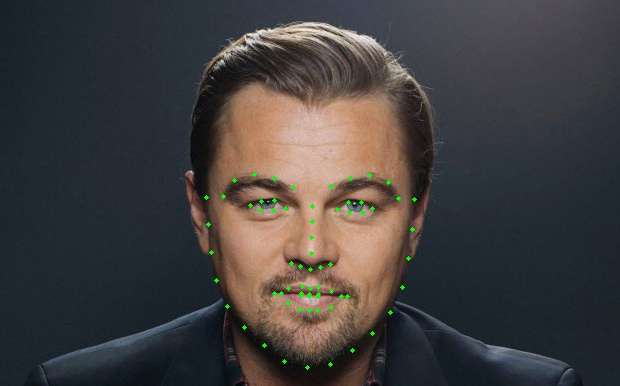
\includegraphics[width=.9\textwidth]{1.jpg}
	\end{subfigure}%
	\begin{subfigure}{0.5\textwidth}
		\centering
		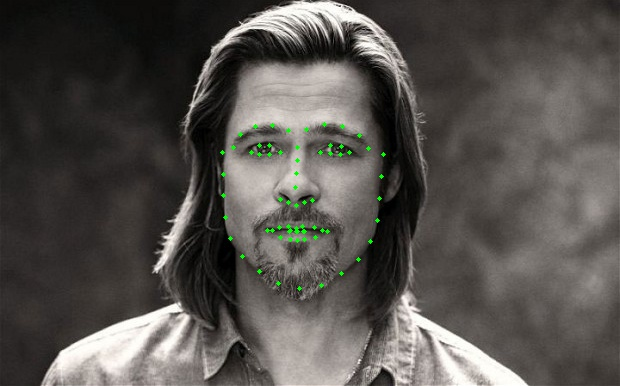
\includegraphics[width=.9\textwidth]{2.jpg}
	\end{subfigure}%
\end{figure}
بردار جا‌به‌جایی بین هر کدام از این 
\lr{key point}‌ها
و 
\lr{key point}
متناظرش در تصویر دوم را محاسبه می‌کنیم و با توجه به تعداد فریم‌های میانی که می‌خواهیم داشته باشیم با استفاده از 
\lr{linear interpolation}
مختصات 
\lr{key point}‌ها 
را برای فریم‌های میانی به دست می‌آوریم.
\begin{figure}[H]
	\centering
	\begin{subfigure}{0.8\textwidth}
		\centering
		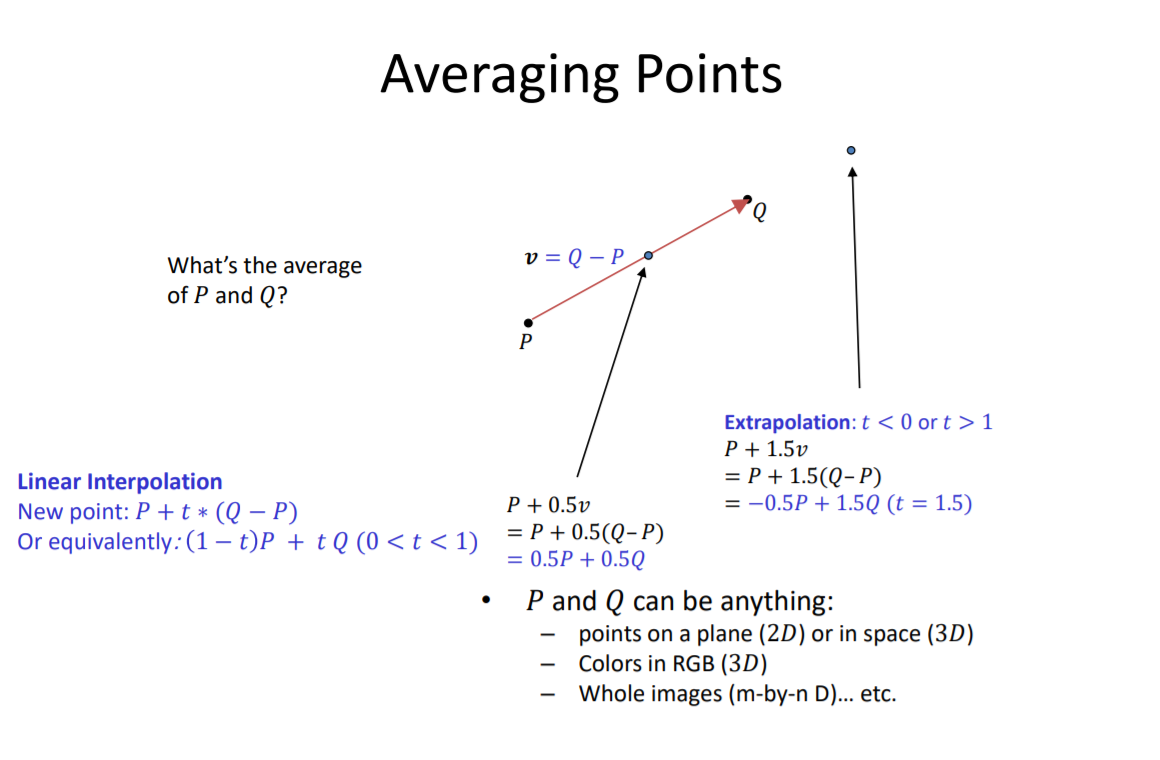
\includegraphics[width=.9\textwidth]{3.png}
	\end{subfigure}
\end{figure}
در مرحله بعد روی دو تصویر مثلث‌بندی انجام می‌دهیم. برای مثلث‌بندی از الگوریتم 
\lr{Delaunay}
که در کتابخانه 
\lr{scipy.spatial}
پیاده‌سازی شده است استفاده می‌کنیم. فقط باید به این نکته دقت کرد که مثلث‌بندی‌ها در دو تصویر متناظر باشند. برای اینکه مثلث‌بندی‌ها متناظر باشد، یک مثلث بندی روی تصویر اول انجام می‌دهیم و همان مثلث‌بندی را به مثلث دوم منتقل می‌کنیم.همانظور که در تصاویر زیر مشاهده می‌کنید، 8 نقطه علاوه بر 
\lr{facial landmarks}
به 
\lr{key points}
اضافه می‌کنیم تا همه تصویر به صورت کامل مثلث‌بندی شود.

\begin{figure}[H]
	\centering
	\begin{subfigure}{0.5\textwidth}
		\centering
		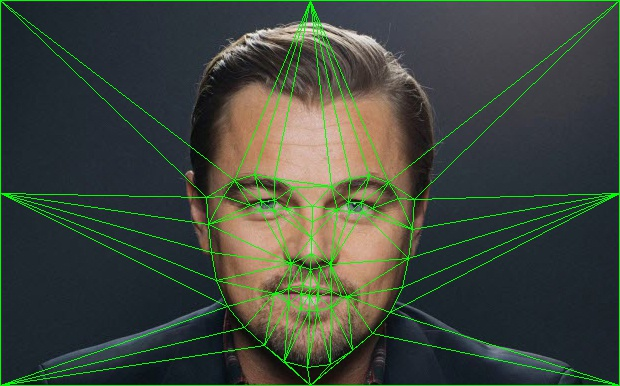
\includegraphics[width=.9\textwidth]{4.jpg}
	\end{subfigure}%
	\begin{subfigure}{0.5\textwidth}
		\centering
		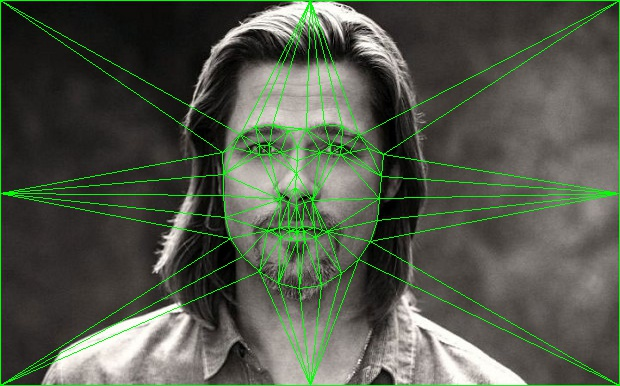
\includegraphics[width=.9\textwidth]{5.jpg}
	\end{subfigure}%
\end{figure}
این مثلث‌بندی را برای فریم‌های میانی هم استفاده می‌کنیم. اگر تعداد نقاط متناظر به اندازه کافی زیاد باشد می‌توان بین هر دو مثلث یک نگاشت هندسی ساده در نظر گرفت که این دو مثلث را به هم متناظر تبدیل بکند. با استفاده از رئوس مثلث‌ها نگاشت ها را محاسبه می‌کنیم و همه نقاط داخل مثلث را در فریم‌های میانی را با این نگاشت‌ها از مثلث متناظر در تصویر اول و در تصویر دوم به دست می‌آوریم.

مراحلی که توضیح داده شد به صورت خلاصه در شکل زیر آمده است.
\begin{figure}[H]
	\centering
	\begin{subfigure}{0.8\textwidth}
		\centering
		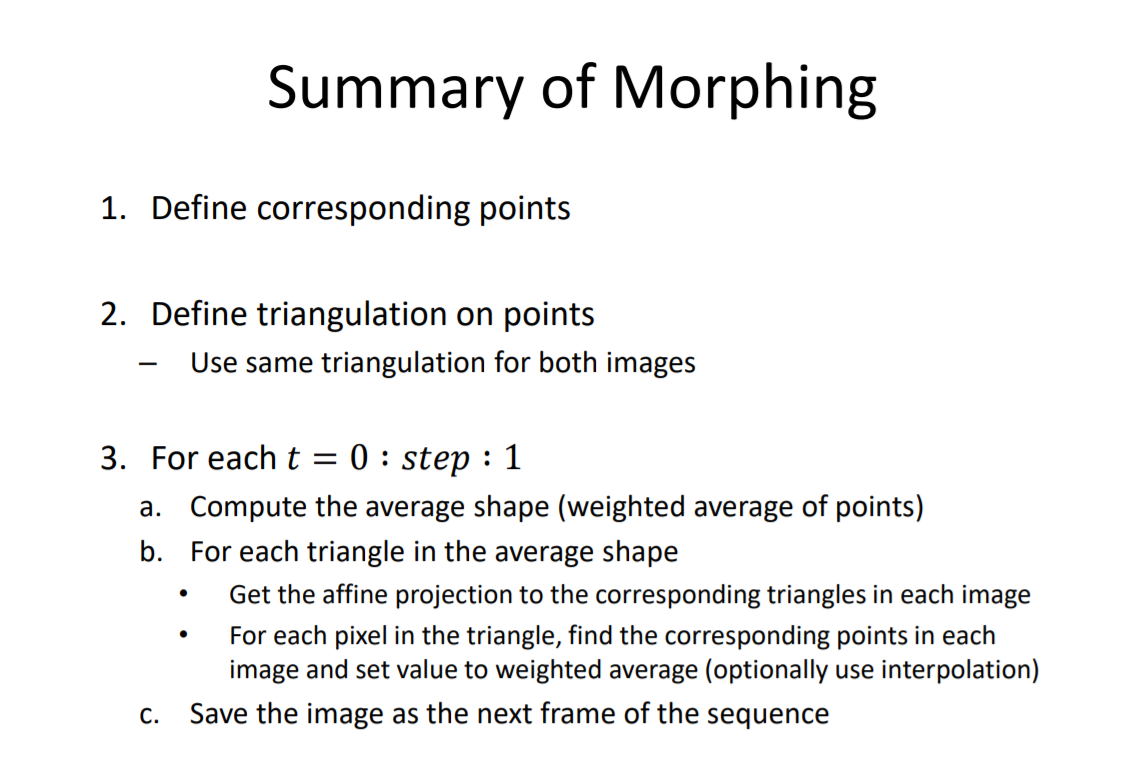
\includegraphics[width=.9\textwidth]{6.png}
	\end{subfigure}
\end{figure}
\section*{توضیح کد.}
برنامه در مجموع حاوی 2 فایل با فرمت
\lr{.py}
می‌باشد که توضیحات هر فایل در پایین آمده است.
\subsection*{$\circ$ utilities.py}
\subsubsection*{\lr{get\_facial\_landmarks(face\_image)}}
این تابع یک تصویر که عکس چهره‌ی یک فرد است را به عنوان ورودی می‌گیرد و با استفاده از کتابخانه‌ی 
\lr{dlib}،
\lr{facial landmark}‌هایِ
چهره به علاوه‌ی 8 نقطه که مشابه شکل زیر در اطراف تصویر در نظرگرفته می‌شود را به عنوان 
\lr{key points}
بر می‌گرداند. 
\begin{figure}[H]
	\centering
	\begin{subfigure}{0.6\textwidth}
		\centering
		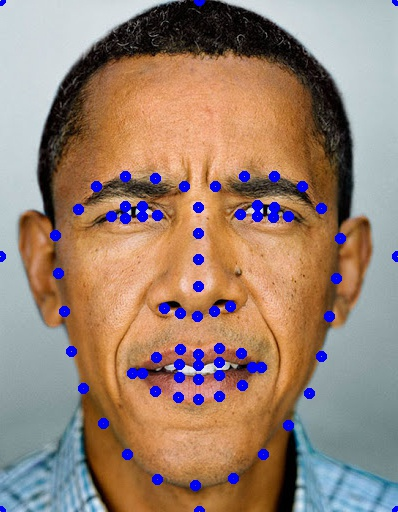
\includegraphics[width=.5\textwidth]{6.jpg}
	\end{subfigure}
\end{figure}
\subsubsection*{\lr{get\_triangulation(facial\_landmarks)}}
این تابع مجموعه نقاطِ
\lr{facial\_landmarks}
را به عنوان ورودی می‌گیرد و با استفاده از الگوریتم
\lr{Delaunay}
که در کتابخانه 
\lr{scipy.spatial}
پیاده‌سازی شده است یک مثلث‌بندی روی این مجموعه نقاط اعمال می‌کند و این مثلث بندی را به عنوان خروجی تابع بر‌می‌گرداند. (مشابه تصویر زیر)
\begin{figure}[H]
	\centering
	\begin{subfigure}{0.6\textwidth}
		\centering
		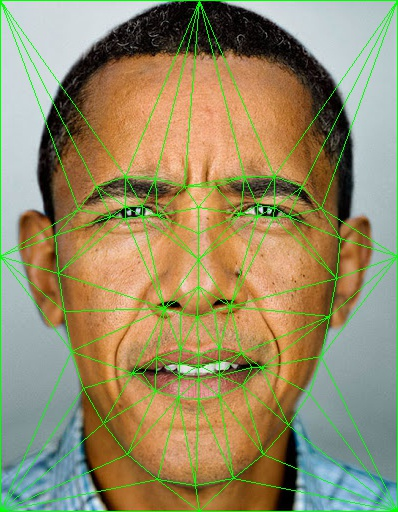
\includegraphics[width=.5\textwidth]{7.jpg}
	\end{subfigure}
\end{figure}
\subsubsection*{\lr{rect\_contains(rect, point)}}
این تابع یک مستطیل و یک نقطه به عنوان ورودی می‌گیرد و در خروجی مشخص می‌کند که آیا نقطه داخل مستسیل قرار می‌گیرد یا نه.
\subsubsection*{\lr{draw\_delaunay\_triangulation(src\_image, facial\_landmarks, triangulation)}}
این تابع یک تصویر، یک مجموعه نقاط و یک مثلث بندی روی این مجموعه نقاط را به عنوان ورودی می‌گیرد و این مثلث بندی را روی تصویر رسم می‌کند.
\subsubsection*{\lr{morph(first\_image, last\_image, facial\_landmarks1, facial\_landmarks2, triangulation, Num\_of\_frames)}}
در این تابع یک حلقه به تعداد فریم‌هایی که می‌خواهیم داشته باشیم اجرا می‌شود و در هر بار اجرا یک فریم میانی را تولید می‌کند و در مسیر
\lr{EX4\_Q2/results/}
ذخیره می‌کند. به این صورت که روی مثلث‌بندی‌ای که به عنوان ورودی به تابع داشته شده است پیمایش می‌کنیم و در هر پیمایش حلقه‌یِ داخلی یک مثلث را در نظر‌ می‌گیرد و مختصات نقاطِ رئوس این مثلث را در تصویر اول محاسبه می‌کند سپس مستطیلِ محیط بر این مثلث را محاسبه می‌کند و در متغیر 
\lr{face1\_triangle\_boundary} 
قرار می‌دهد، 
\lr{cropped\_face1\_triangle\_boundary}
آن مستطیل از تصویرِ اول است که به مثلث در تصویر اول محیط شده است. در ادامه مختصات نقاطِ رئوس این مثلث را در تصویر دوم محاسبه می‌کند سپس مستطیلِ محیط بر این مثلث را در تصویر دوم محاسبه می‌کند و در متغیر 
\lr{face1\_triangle\_boundary} 
قرار می‌دهد، 
\lr{cropped\_face1\_triangle\_boundary}
آن مستطیل از تصویرِ دوم است که به مثلث در تصویر دوم محیط شده است. با استفاده از 
\lr{face1\_triangle}
و
\lr{face2\_triangle}
و با روش 
\lr{linear interpolation}
مختصات رئوس این مثلث را در فریم میانی محاسبه ‌می‌کند و در متغیر 
\lr{middle\_frame\_triangle}
ذخیره می‌کند.
\begin{figure}[H]
	\centering
	\begin{subfigure}{0.5\textwidth}
		\centering
		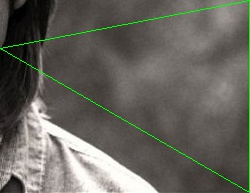
\includegraphics[width=.5\textwidth]{cropped_face1_triangle_boundary.jpg}
		\subcaption{cropped\_face1\_triangle\_boundary}
	\end{subfigure}%
	\begin{subfigure}{0.5\textwidth}
		\centering
		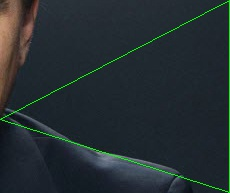
\includegraphics[width=.5\textwidth]{cropped_face2_triangle_boundary.jpg}
		\subcaption{cropped\_face2\_triangle\_boundary}
	\end{subfigure}%
	
\end{figure}
 با استفاده از تابع 
\lr{fillConvexPloy}
یک 
\lr{mask}
برای مثلث میانی همانند تصویر زیر به دست می‌آورد.	
\begin{figure}[H]
	\centering
	\begin{subfigure}{0.6\textwidth}
		\centering
		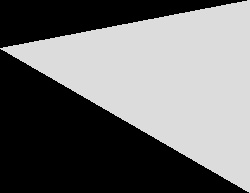
\includegraphics[width=.5\textwidth]{cropped_middle_frame_triangle_mask.jpg}
	\end{subfigure}
\end{figure}
در ادامه با استفاده از تابع 
\lr{cv.getAffineTransform}
نگاشت بینِ مثلث تصویر اول و مثلث میانی و نگاشت بین مثلث تصور آخر و مثلث میانی را به دست می‌آورد و با استفاده از تابع 
\lr{cv.warpAffine}
این نگاشت‌ها را روی 
\lr{cropped\_face1\_triangle\_boundary}
و
\lr{cropped\_face2\_triangle\_boundary}
اعمال می‌کند و در نهایت 
\lr{cropped\_middle\_frame\_triangle\_mask}
را روی نتایج با استفاده از تابع 
\lr{cv.bitwise\_and}
اعمال می‌کند و نتایج به دست آمده را با روش 
\lr{linear interpolation}
با هم جمع کرده تا شکلی مشابه تصویر زیر حاصل شود. 
\begin{figure}[H]
	\centering
	\begin{subfigure}{0.6\textwidth}
		\centering
		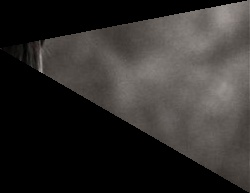
\includegraphics[width=.5\textwidth]{middle_triangle.jpg}
	\end{subfigure}
\end{figure}
در آخر هم آن قسمت از 
\lr{middle\_triangle}
که با تصویری که تا به اینجا ساخته شده اشتراک ندارد را در 
\lr{result}
قرار می‌دهد.

\subsection*{$\circ$ q2.py}

در این فایل ابتدا تصاویر
\lr{BradPitt.jpg}
و
\lr{DiCaprio.jpg}
از مسیر 
\lr{EX4\_Q2/images/}
لود می‌شود و در ادامه با استفاده از تابع 
 \lr{get\_facial\_landmarks}
 ، 
 \lr{facial landmark}‌هایِ
 دو تصویر محاسبه می‌شود و بعد از اینکه مثلث‌بندی محاسبه شد با فراخوانی تابع 
 \lr{morph}
 ،
 \lr{morphing}
 انجام می‌شود و نتایج در مسیر
 \lr{EX4\_Q2/results/}
 ذخیره می‌شود.


\end{document}
